%!TeX root=../main.tex

\chapter{Conceitos}
\label{cap:conceitos}

\section{Isometria}
\label{sec:isometria}

A projeção isométrica é um caso particular da projeção ortogonal que permite a representação
gráfica tridimensional em superfícies bidimensionais. Matematicamente, a isometria é
caracterizada pelo alinhamento dos eixos coordenados (\textbf{X}, \textbf{Y} e \textbf{Z}) em relação ao plano de
projeção, de modo que os ângulos formados entre a projeção de cada par de eixos sejam
exatamente iguais a 120$\degree$. Essa propriedade garante que a escala de medida permaneça
uniforme ao longo de todos os eixos, eliminando os pontos de fuga característicos da
perspectiva cônica, que é a forma como o olho humano enxerga a realidade.

\begin{figure}[H]
	\centering
	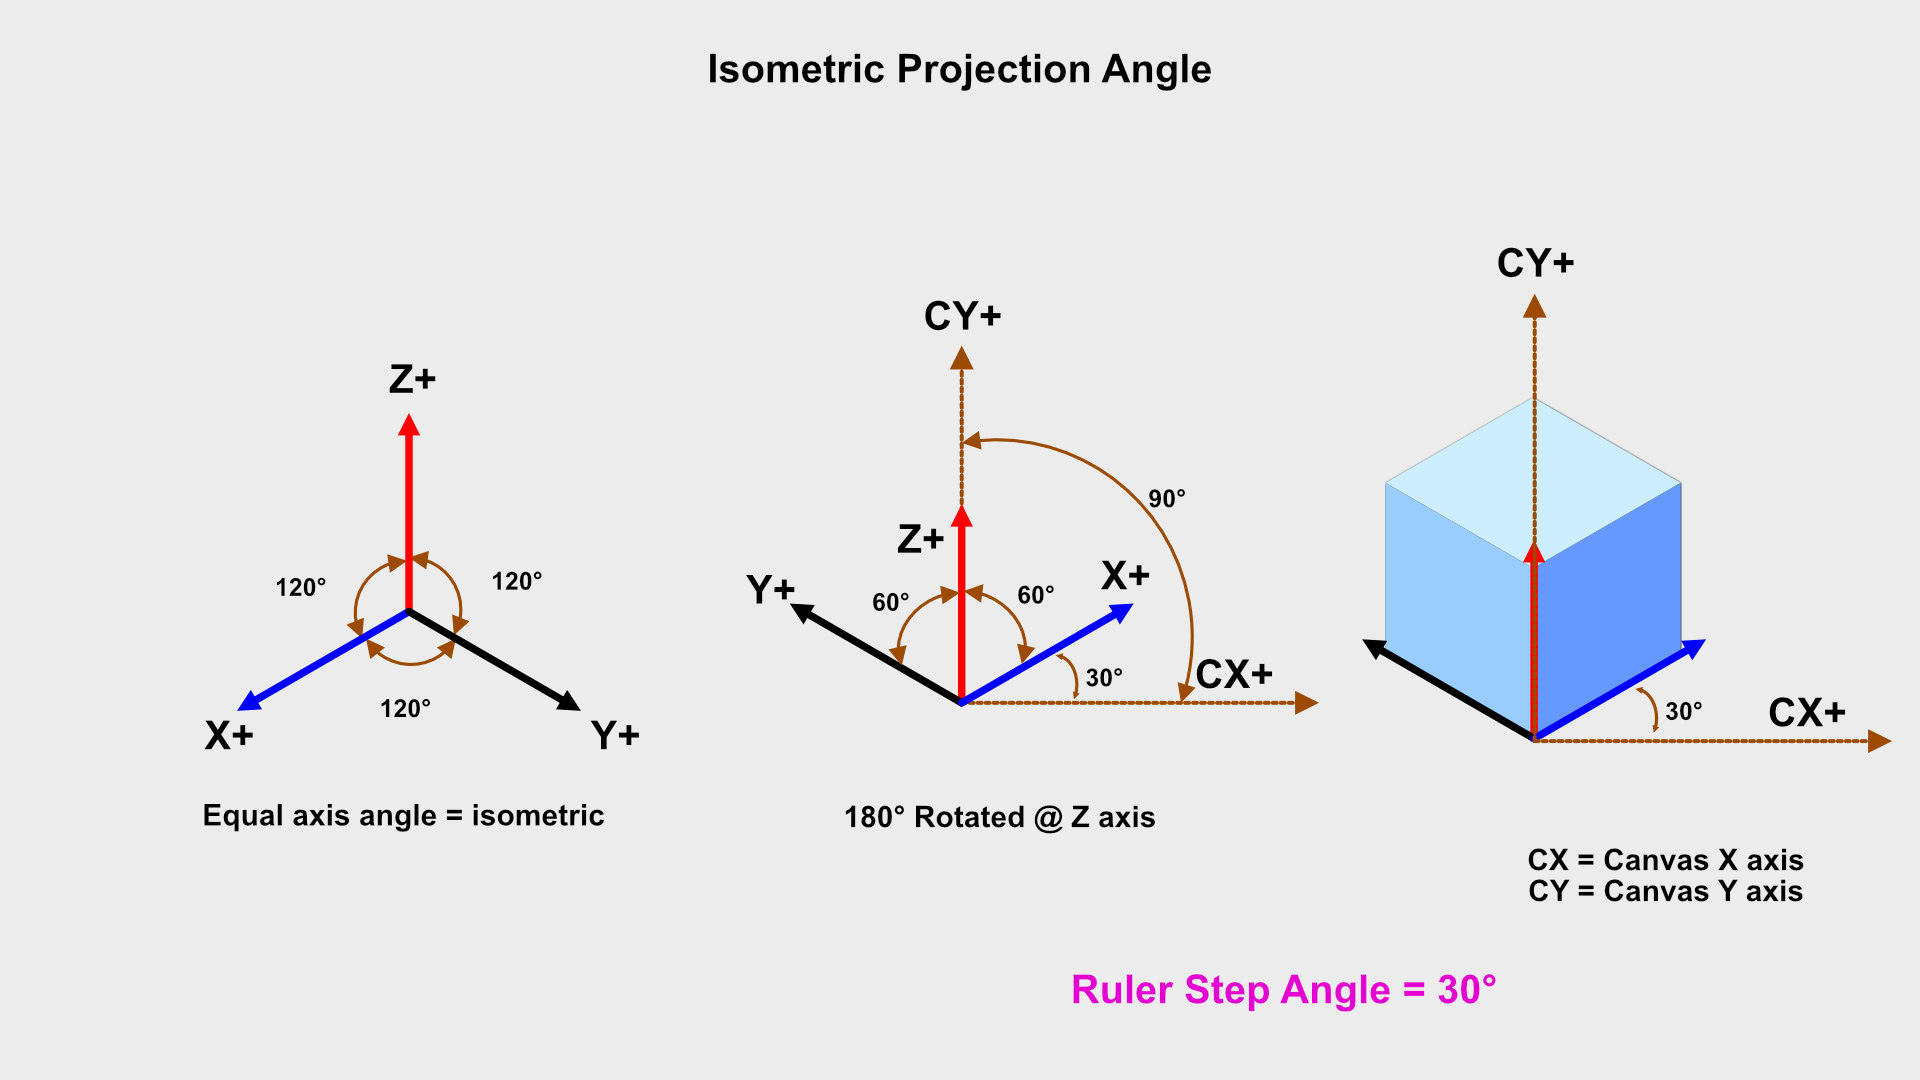
\includegraphics[width=0.7\textwidth]{isometric-120}
	\caption{Eixos X, Y e Z em uma projeção isométrica em relação ao canvas. Fonte: \cite{isometric-120}}\label{fig:isometric-120}
\end{figure}

Historicamente, o uso da perspectiva isométrica na indústria de jogos eletrônicos surgiu no
início da década de 1980 como uma solução para contornar limitações computacionais dos
hardwares da época. Antes do surgimento das unidades de processamento gráfico (GPUs)
dedicadas ao 3D em tempo real, renderizar polígonos tridimensionais complexos era inviável.
Os desenvolvedores passaram, então, a utilizar \textit{sprites} bidimensionais desenhados em ângulo
isométrico, popularizando a clássica proporção de inclinação de 2:1 em \textit{pixel art}, o que
permitia criar uma ilusão de profundidade e volume sem o custo computacional de cálculos de
perspectiva.

Todavia, esta proporção 2:1 não é uma projeção isométrica verdadeira. A projeção isométrica é um
tipo de projeção axonométrica, que é uma categoria mais ampla de projeções ortogonais (paralelas).
Nessas projeções, os ângulos entre os eixos podem variar, mas por serem projeções paralelas,
elas eliminam os pontos de fuga característicos da perspectiva cônica. A projeção axonométrica
é subdividida em três tipos:

\begin{description}
	\item[Isométrica] Caracteriza-se pela igualdade perfeita entre os ângulos formados pelos três eixos,
	cada um medindo exatamente $120^\circ$ entre si (com uma inclinação de $30^\circ$ em relação à linha
	horizontal de referência). Essa propriedade garante que a escala espacial e o fator de proporção sejam
	idênticos ao longo de todas as dimensões;
	\item[Dimétrica] Apresenta dois ângulos iguais entre a projeção dos eixos e um ângulo distinto,
	resultando em duas escalas de medição idênticas e uma terceira diferente.
	\item[Trimétrica] Todos os três ângulos entre os eixos são diferentes entre si.
\end{description}

\begin{figure}[H]
	\centering
	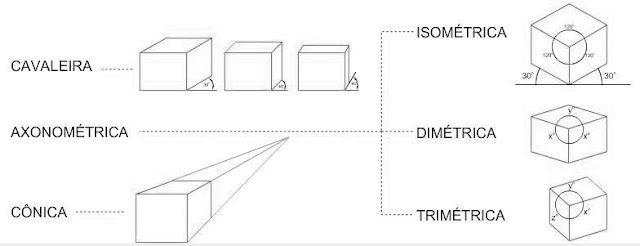
\includegraphics[width=0.8\textwidth]{axonometria}
	\caption{Tipos de perspectivas mais utilizadas. Fonte: \cite{axonometric}}\label{fig:axonometric}
\end{figure}

Ou seja, em uma perspectiva isométrica perfeita ($120^\circ$), a linha diagonal sobe a um ângulo exato
de $30^\circ$ ($\tan(30^\circ) \approx 0{,}577$). Na era da \textit{pixel art}, traçar uma linha com inclinação de $30^\circ$ era
impossível sem gerar \textit{aliasing} (serrilhamento irregular) pesado na tela. Para resolver isso, os desenvolvedores
criaram a regra prática de ``andar'' 2 \textit{pixels} na horizontal para 1 \textit{pixel} na vertical, resultando em uma inclinação de $26{,}565^\circ$
($\arctan(0{,}5) = 26{,}565^\circ$), que é a proporção 2:1. Como essa inclinação não é exatamente $30^\circ$, os ângulos entre os
eixos tornam-se aproximadamente $116{,}565^\circ$, $116{,}565^\circ$ e $126{,}87^\circ$, o que caracteriza uma projeção dimétrica, 
mas que ainda é comumente referida como isométrica na indústria de jogos eletrônicos pois a simula muito bem visualmente.

Os principais marcos durante o pioneirismo desta técnica foram os jogos \textit{Zaxxon} (1982), \textit{Ant Attack} (1983)
e \textit{Knight Lore} (1984):

\begin{description}
	\item[\textit{Zaxxon} (1982):] É um jogo de tiro espacial onde o jogador pilota uma nave em uma
	base inimiga com movimento baseado em rolagem diagonal, sendo também um dos primeiros jogos a
	exibir sombras na tela, para indicar a posição da nave em relação à superfície. Desenvolvido pela
	SEGA em 1982, é amplamente reconhecido como o primeiro jogo eletrônico a empregar a projeção
	axonométrica, que inclusive dá nome ao jogo (\textit{AXXON} vem de \textit{AXONométrica}).
	\begin{figure}[H]
		\centering
		\begin{subfigure}{0.4\textwidth}
			\centering
			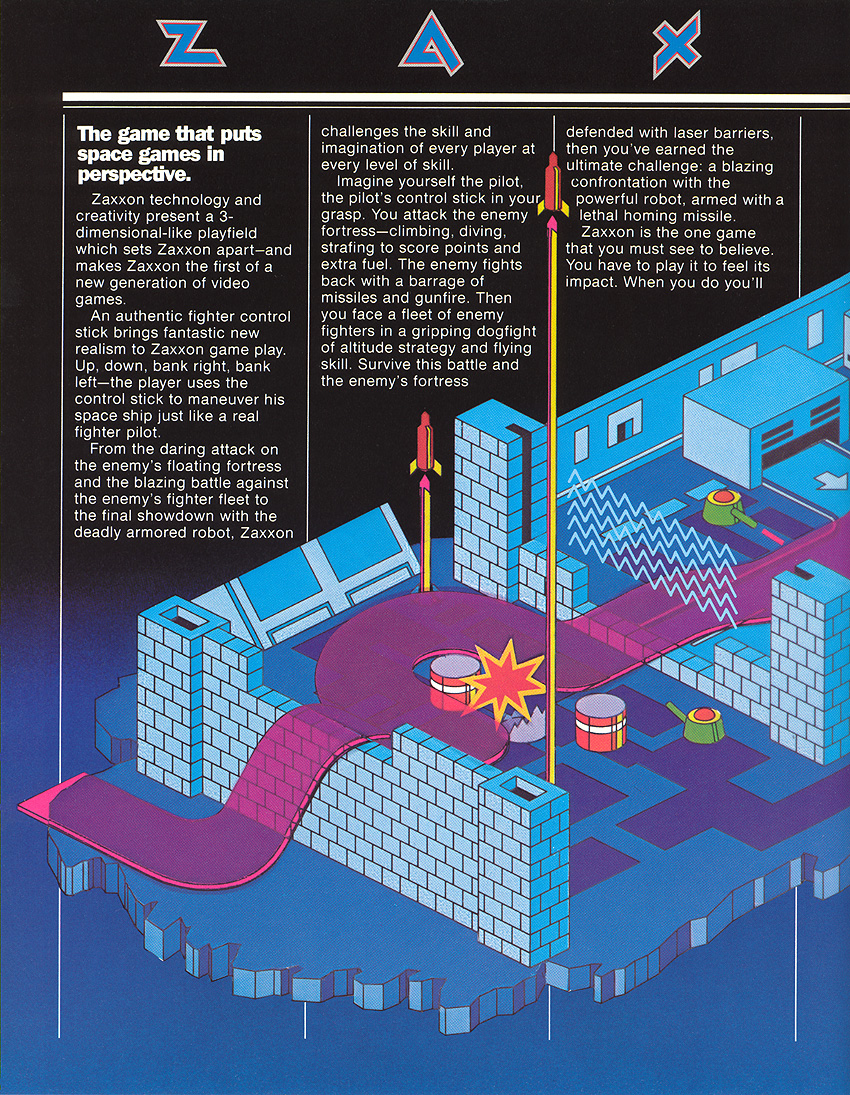
\includegraphics[width=\textwidth]{zaxxon-flyer-a}
			\label{fig:zaxxon:a}
		\end{subfigure}
		\begin{subfigure}{0.4\textwidth}
			\centering
			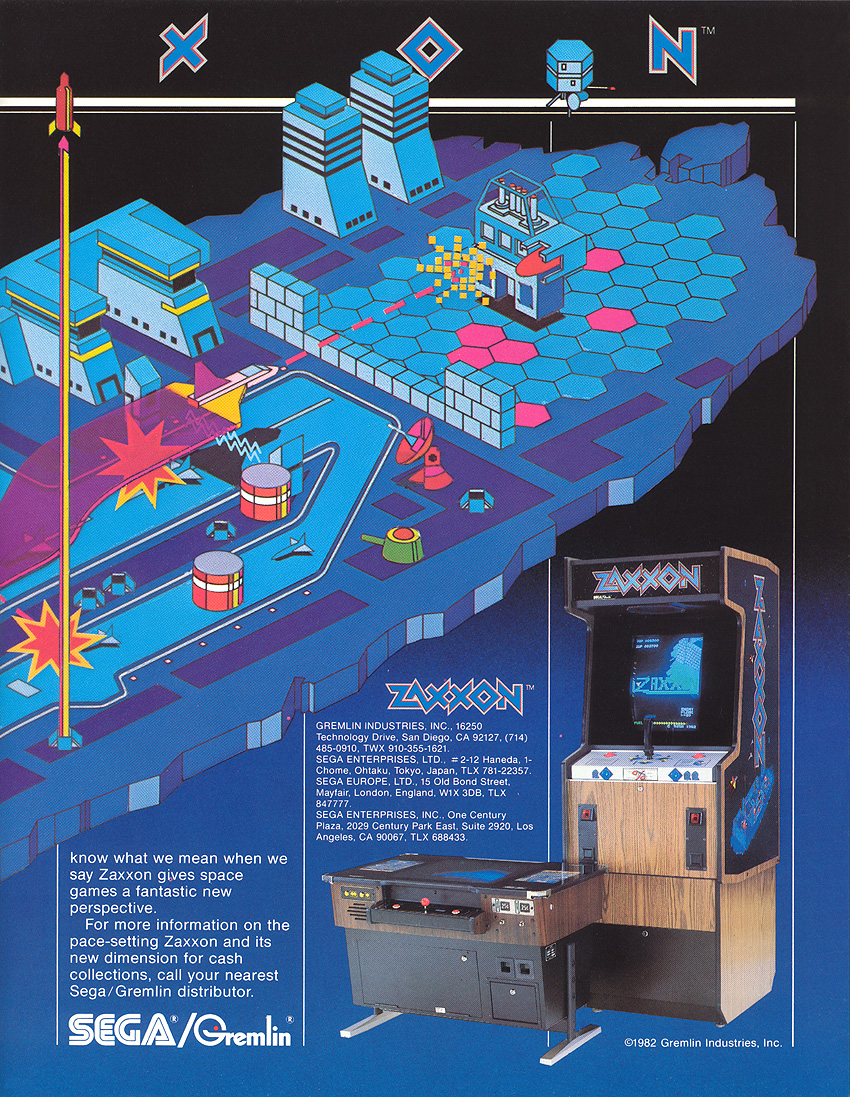
\includegraphics[width=\textwidth]{zaxxon-flyer-b}
			\label{fig:zaxxon:b}
		\end{subfigure}
		\caption{Folheto promocional de Zaxxon para Arcade. Fonte: \cite{zaxxon-flyer}}\label{fig:zaxxon}
	\end{figure}
	\item[\textit{Ant Attack} (1983):] Embora não tenha sido o primeiro jogo isométrico, foi o primeiro
	a adicionar um grau de liberdade vertical, permitindo que o jogador pudesse se mover livremente
	também para cima e para baixo, ao invés de apenas norte, sul, leste e oeste. Sendo talvez o primeiro
	jogo isométrico para computadores pessoais e também um dos primeiros a permitir que o jogador escolha
	seu gênero. Desenvolvido em 1983 por Sandy White para o ZX Spectrum, neste jogo o usuário começa
	escolhendo controlar o garoto ou a garota, então entra na cidade fortificada de Antescher para
	salvar o outro que foi capturado e imobilizado em algum lugar da cidade. A cidade é habitada por
	formigas gigantes que perseguem e mordem o jogador, cuja única forma de se defender é arremessando
	granadas que também podem machucar outros humanos. O objetivo do jogo é localizar o refém e escapar
	da cidade.
	\begin{figure}[H]
		\centering
		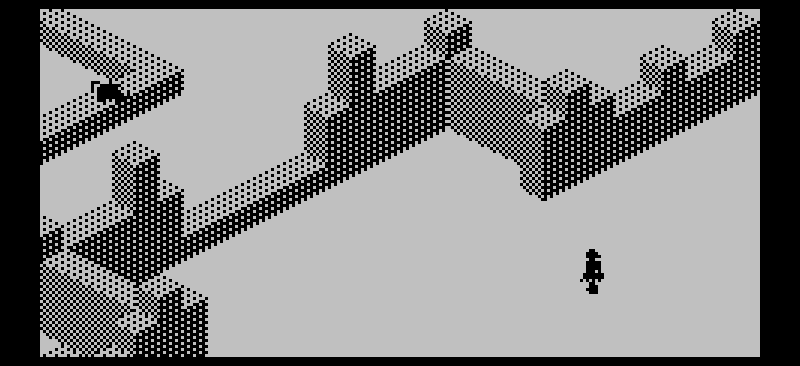
\includegraphics[width=0.7\textwidth]{ant-attack}
		\caption{Tela inicial de Ant Attack. Fonte: \cite{ant-attack}}\label{fig:ant_attack}
	\end{figure}
	\item[\textit{Knight Lore} (1984):] É um jogo de ação e aventura onde o jogador controla o herói
	\textit{Sabreman} (da série que começou com \textit{Sabre Wulf}), que foi mordido e amaldiçoado como lobisomem. Ele
	tem 40 dias para explorar um castelo de 128 salas, resolver quebra-cabeças e preparar um antídoto
	em um caldeirão. Foi um dos responsáveis por popularizar o gênero de aventura isométrica que por
	meio de sua técnica de mascaramento de imagem, chamada de \textit{Filmation}, permitia imagens passarem por
	baixo e por cima uma das outras sem que seus conteúdos colidissem, criando uma ilusão de profundidade
	que não era nativa dos computadores da época. O jogo foi publicado em 1984 e é considerado um trabalho
	seminal na história dos jogos britânicos, sendo coroado Jogo do Ano pela \textit{Golden Joystick Awards} e pela
	\textit{Popular Computing Weekly}, e lembrado como o primeiro jogo que ofereceu um mundo “explorável”, cuja
	influência persiste em jogos de RPG para computador.
	\begin{figure}[H]
		\centering
		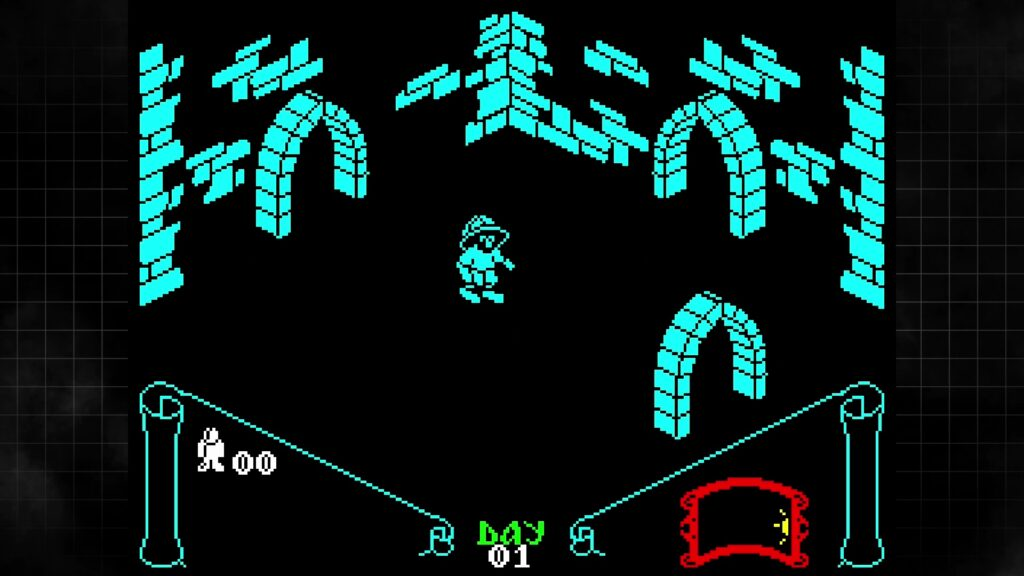
\includegraphics[width=0.7\textwidth]{knight-lore}
		\caption{Knight Lore. Fonte: \cite{knight-lore}}\label{fig:knight_lore}
	\end{figure}

\end{description}

No desenvolvimento moderno, a câmera isométrica é geralmente construída configurando-se
uma câmera 3D com projeção ortográfica alinhada a um ângulo fixo. Do ponto de vista de \textit{game design},
a adoção da câmera isométrica proporciona vantagens diretas para a jogabilidade e percepção do espaço, como:

\begin{description}
	\item[Clareza Espacial e Legibilidade:] Por não apresentar encurtamento perspectivo
	\mbox{(\textit{foreshortening})}, os objetos mantêm a mesma escala visual independentemente da sua
	distância em relação à câmera. Isso facilita a leitura imediata de distâncias, trajetórias e
	posições no cenário.
	\item[Ampla Visão do Cenário:] Permite que o jogador visualize simultaneamente o
	personagem principal, múltiplos inimigos ao redor e perigos do ambiente, favorecendo a
	antecipação de ações e o planejamento de reações.
	\item[Desempenho Visual Uniforme:] A ausência de cálculo de deformação de perspectiva
	simplifica o \textit{culling} de oclusão e otimiza a renderização de elementos estáticos e
	dinâmicos.

\end{description}

No entanto, o uso da isometria introduz desafios específicos que demandam soluções
intencionais de design, como a oclusão de elementos (quando objetos altos do cenário
escondem o personagem ou inimigos atrás deles) e a percepção de altura em saltos. Essas
particularidades exigem um planejamento de \textit{level design} e o uso de \textit{shaders} ou transparências
dinâmicas para preservar a orientação do jogador durante sua navegação pelo mapa. Diferentes jogos resolvem
problemas de isometria de maneiras distintas criativamente e tecnologicamente.

\begin{description}
	\item[Efeito Fantasma] Em jogos como Death's Door (2021) e Tunic (2022), quando o personagem passa atrás
	de uma árvore, parede ou ruína, o jogo utiliza um \textit{shader} de recorte ou transparência que
	desenha uma silhueta do personagem ``atrás'' do obstáculo. Assim, o jogador continua enxergando
	exatamente onde seu personagem está, mesmo com a geometria física bloqueando a visão direta.
	\begin{figure}[H]
		\centering
		\begin{subfigure}{0.48\textwidth}
			\centering
			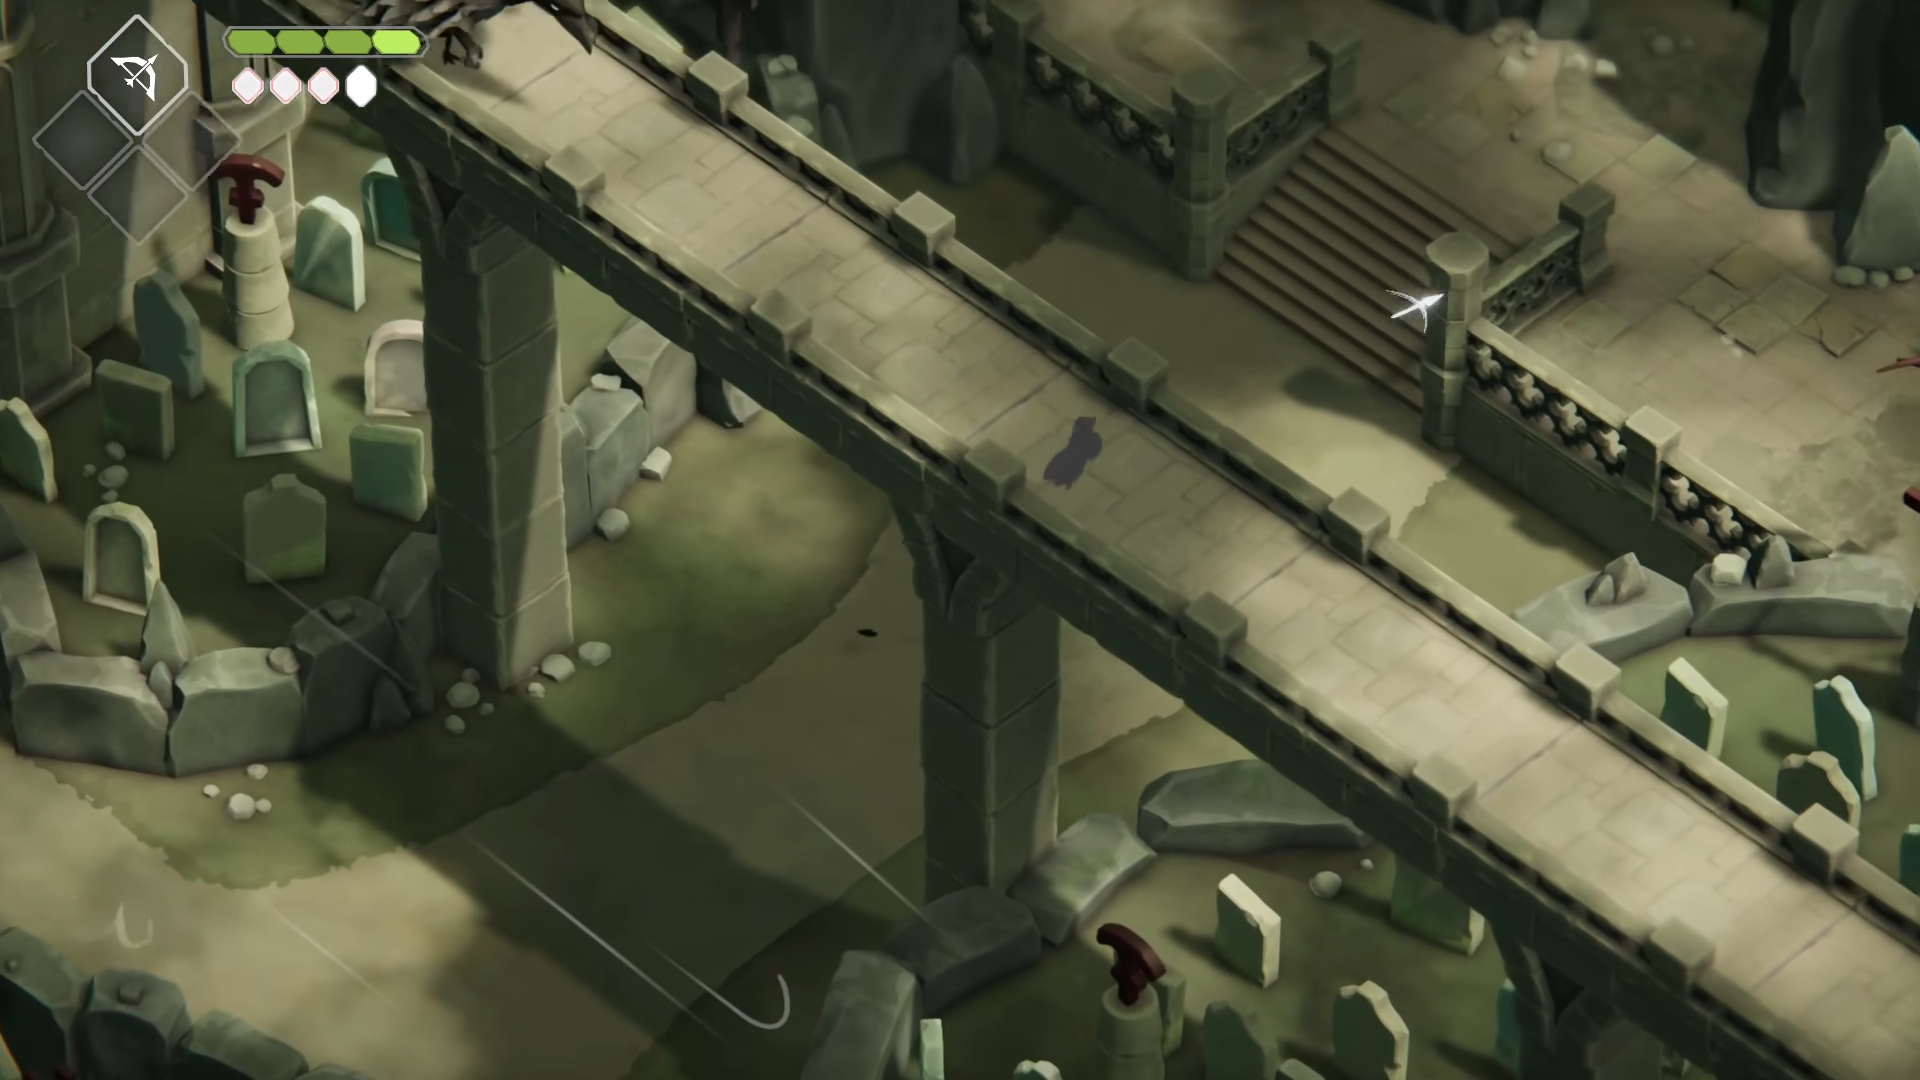
\includegraphics[width=\textwidth]{deaths_door_ghost}
			\caption{Death's Door (2021). Fonte: \cite{deaths-door-game}}\label{fig:ghost_effect_examples:deaths-door}
		\end{subfigure}
		\begin{subfigure}{0.48\textwidth}
			\centering
			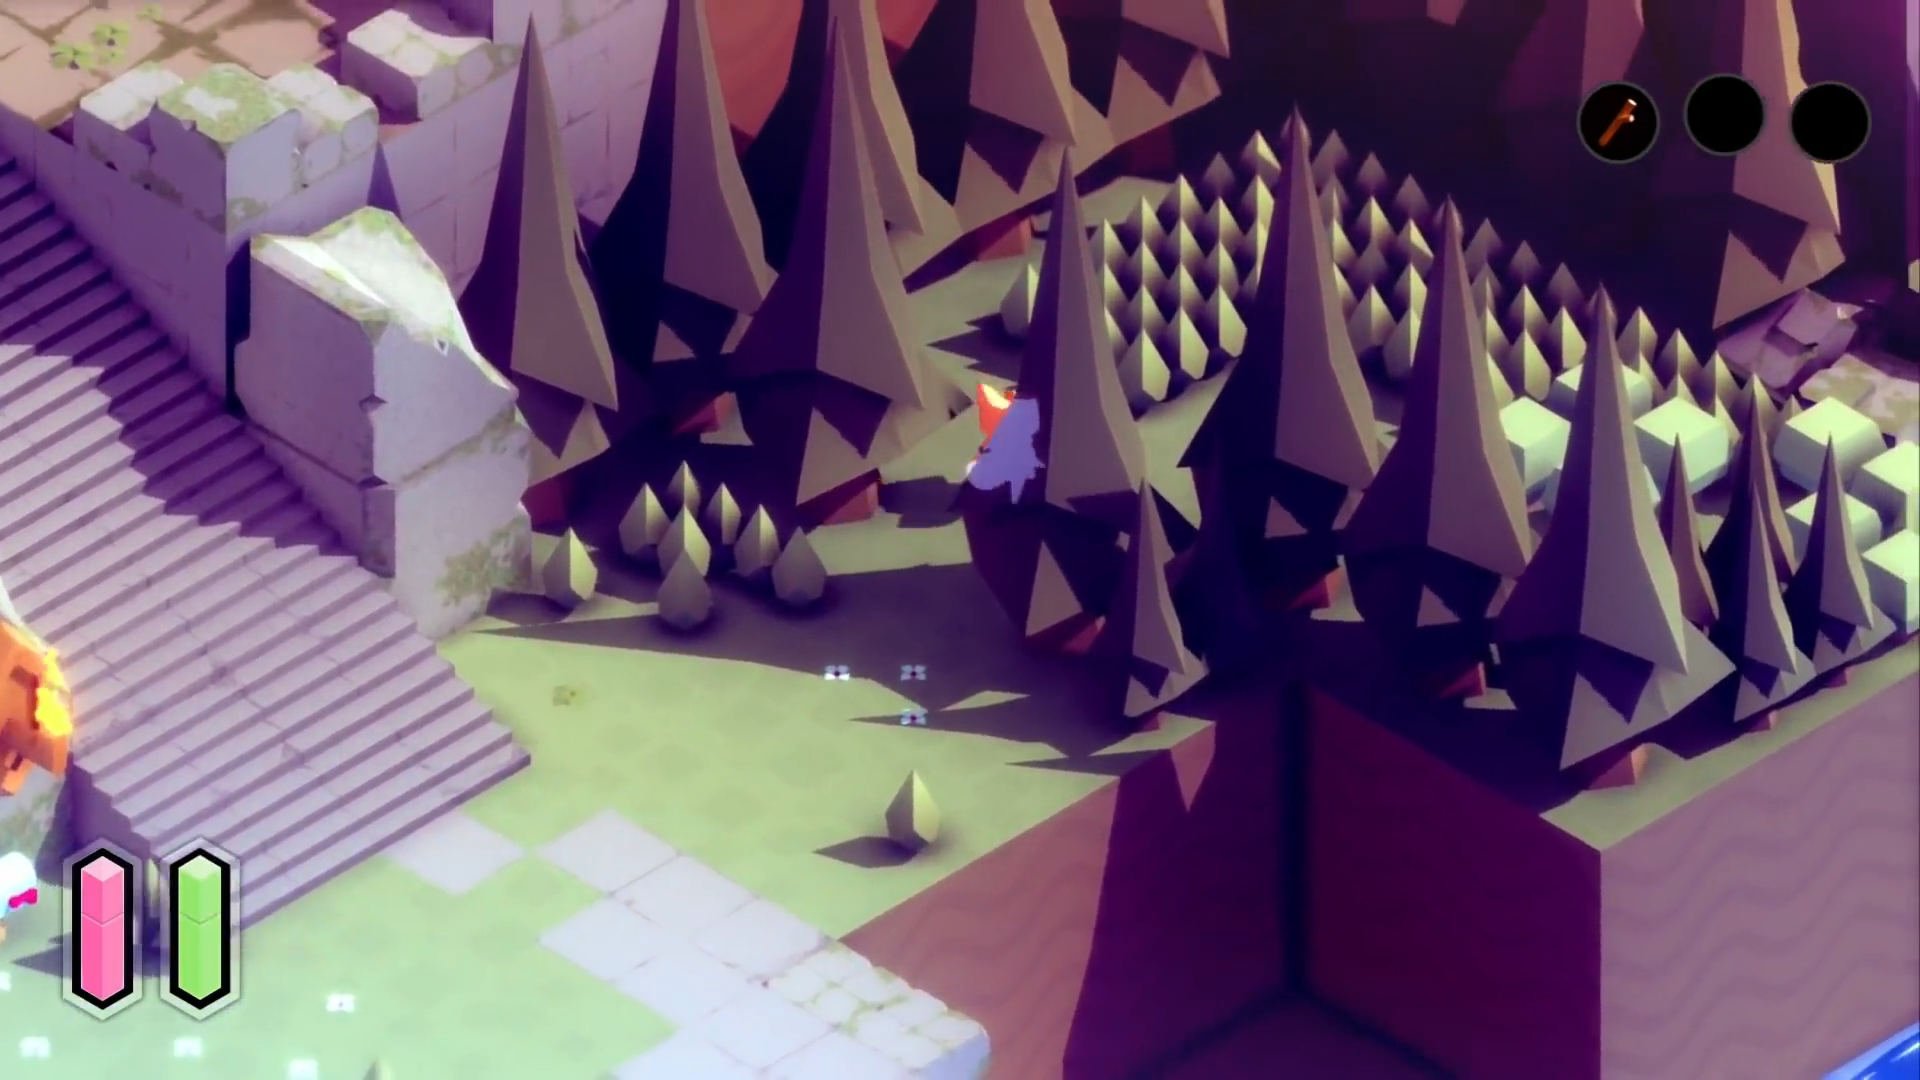
\includegraphics[width=\textwidth]{tunic_ghost}
			\caption{Tunic (2022). Fonte: \cite{tunic-game}}\label{fig:ghost_effect_examples:tunic}
		\end{subfigure}
		\caption{É possível ver a silhueta dos personagens através dos obstáculos.}\label{fig:ghost_effect_examples}
	\end{figure}

	\item[Transparência Dinâmica] Na presença de muitas paredes altas e masmorras como em Diablo IV (2023),
	quando o personagem se posiciona atrás de uma parede vertical em relação à câmera, um \textit{shader}
	de transparência acionado por \textit{raycasting}/linha de visão faz a parede desvanecer ou se dissolver
	completamente, revelando o espaço oculto.

	\begin{figure}[H]
		\centering
		\begin{subfigure}{0.48\textwidth}
			\centering
			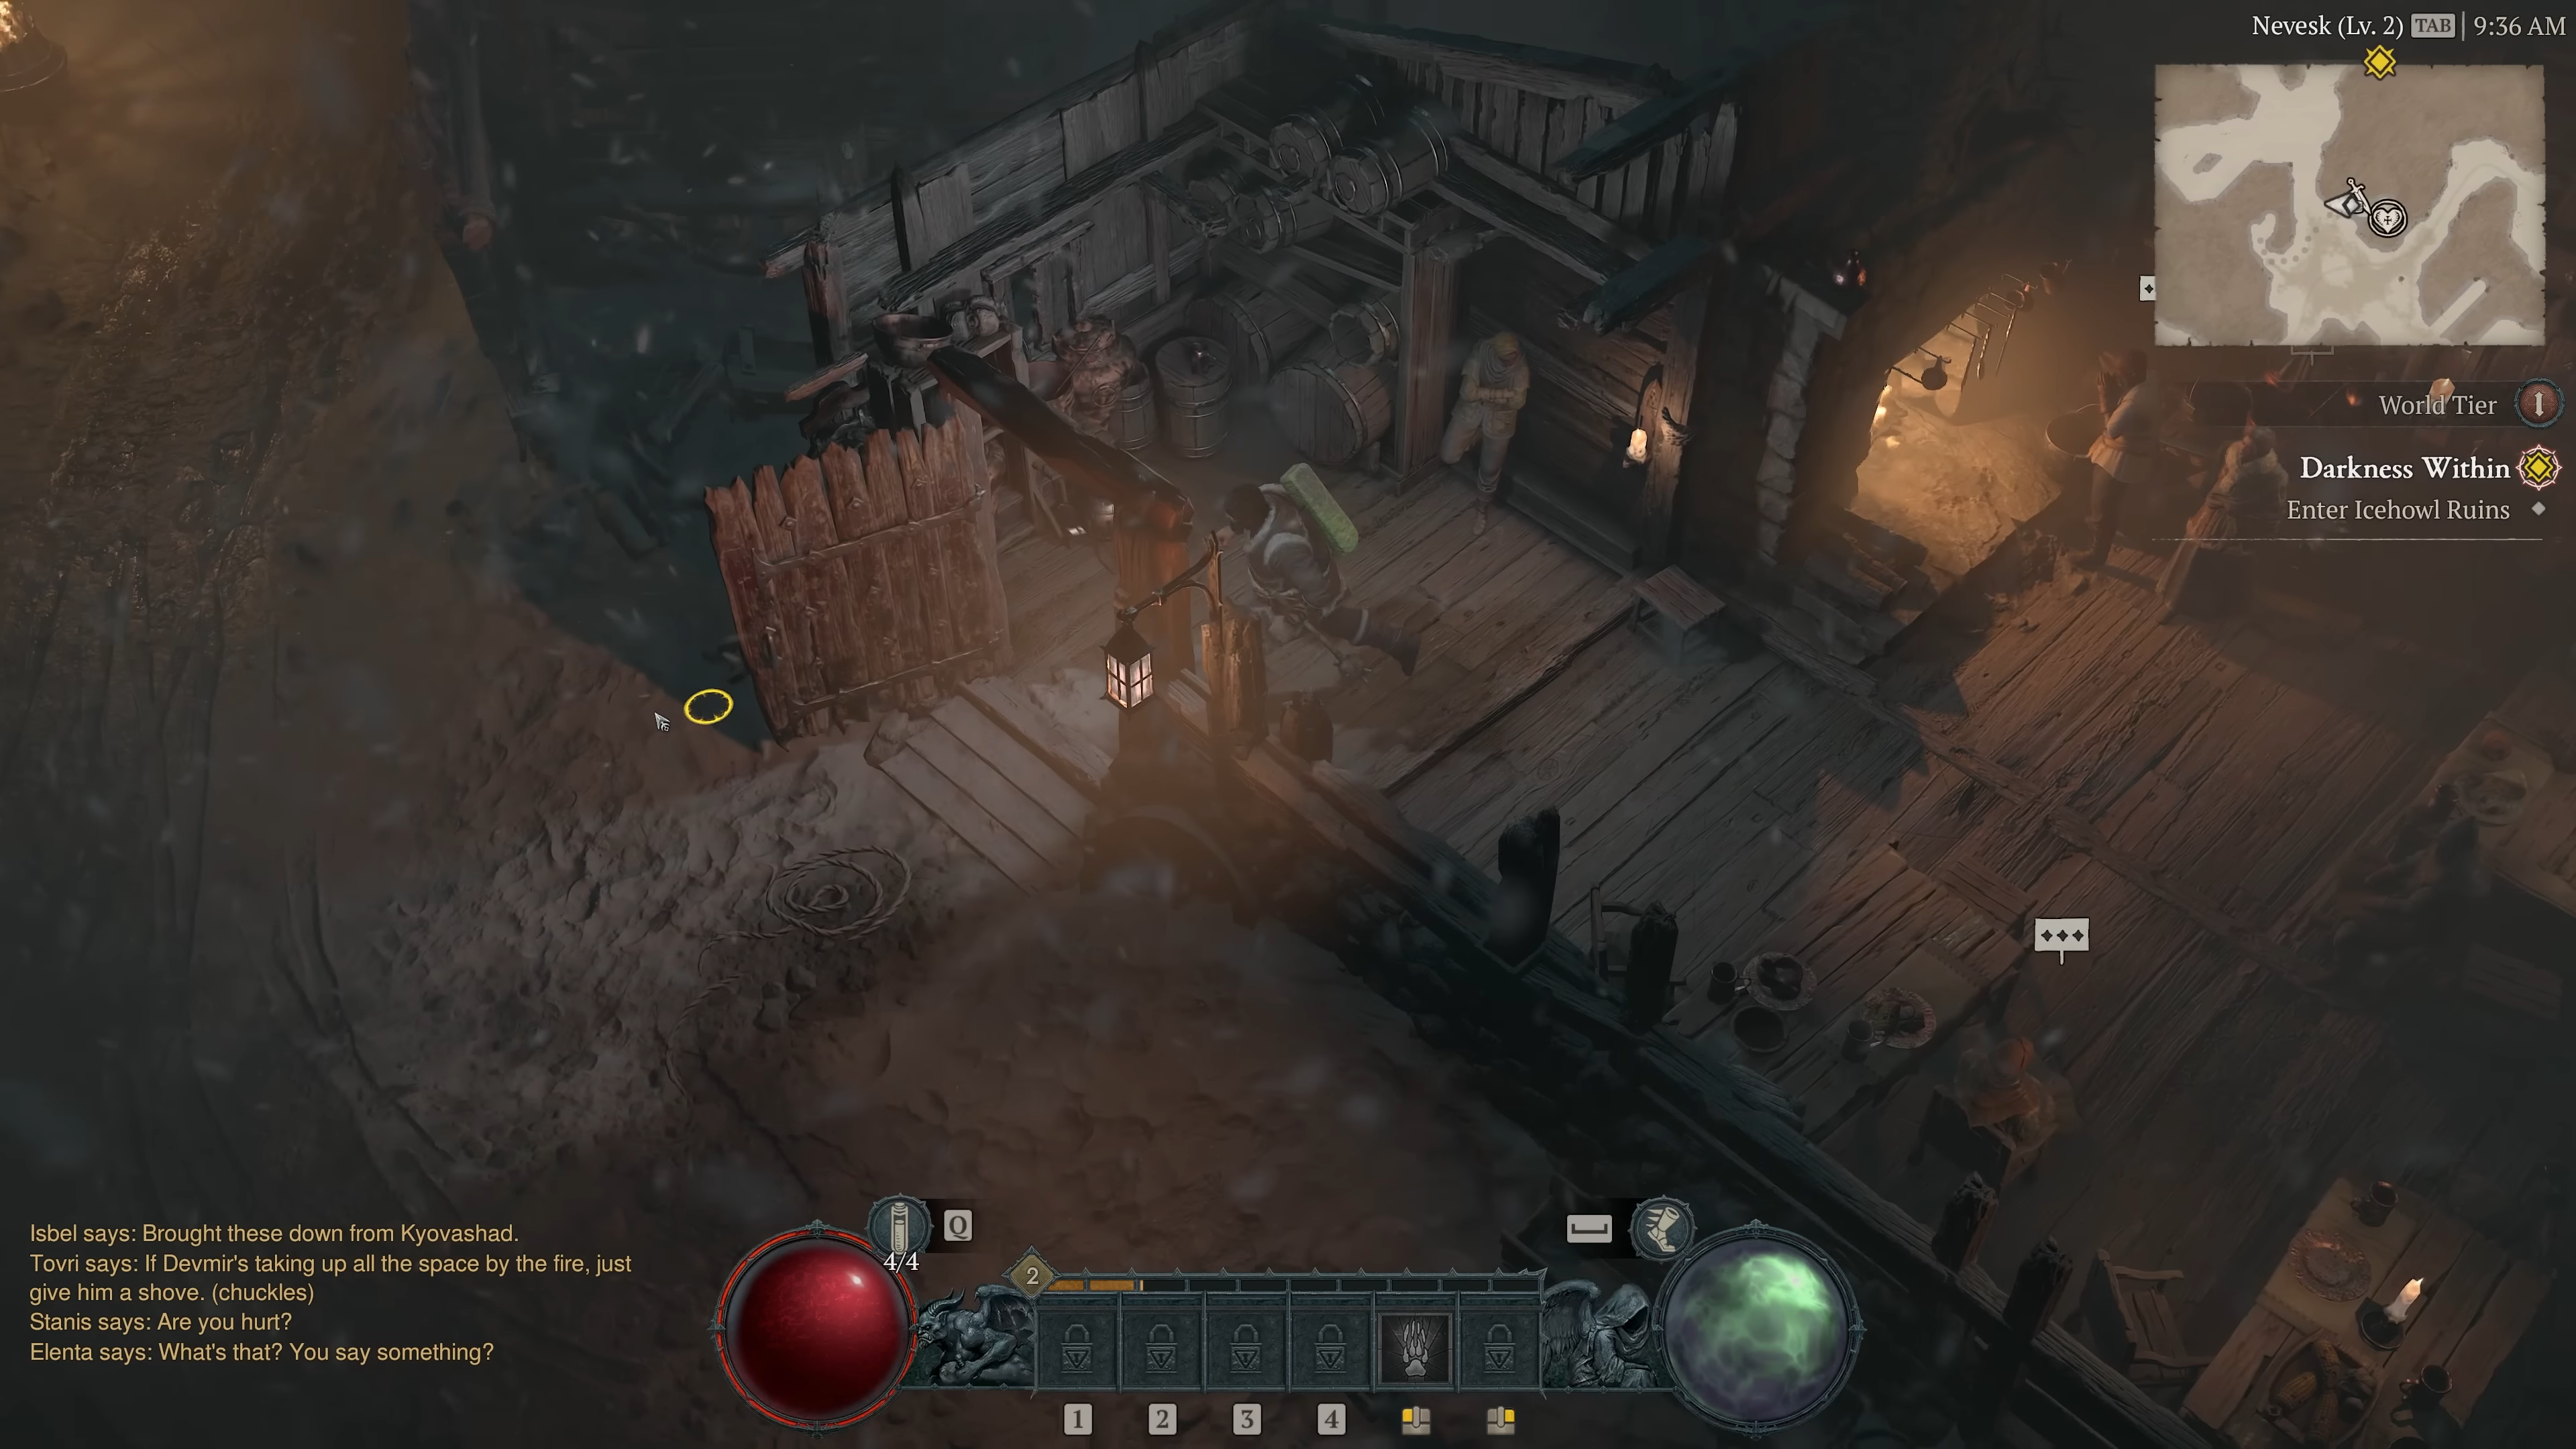
\includegraphics[width=\textwidth]{diablo_inside}
			\caption{Visão interna da casa.}\label{fig:fade_out_example:a}
		\end{subfigure}
		\begin{subfigure}{0.48\textwidth}
			\centering
			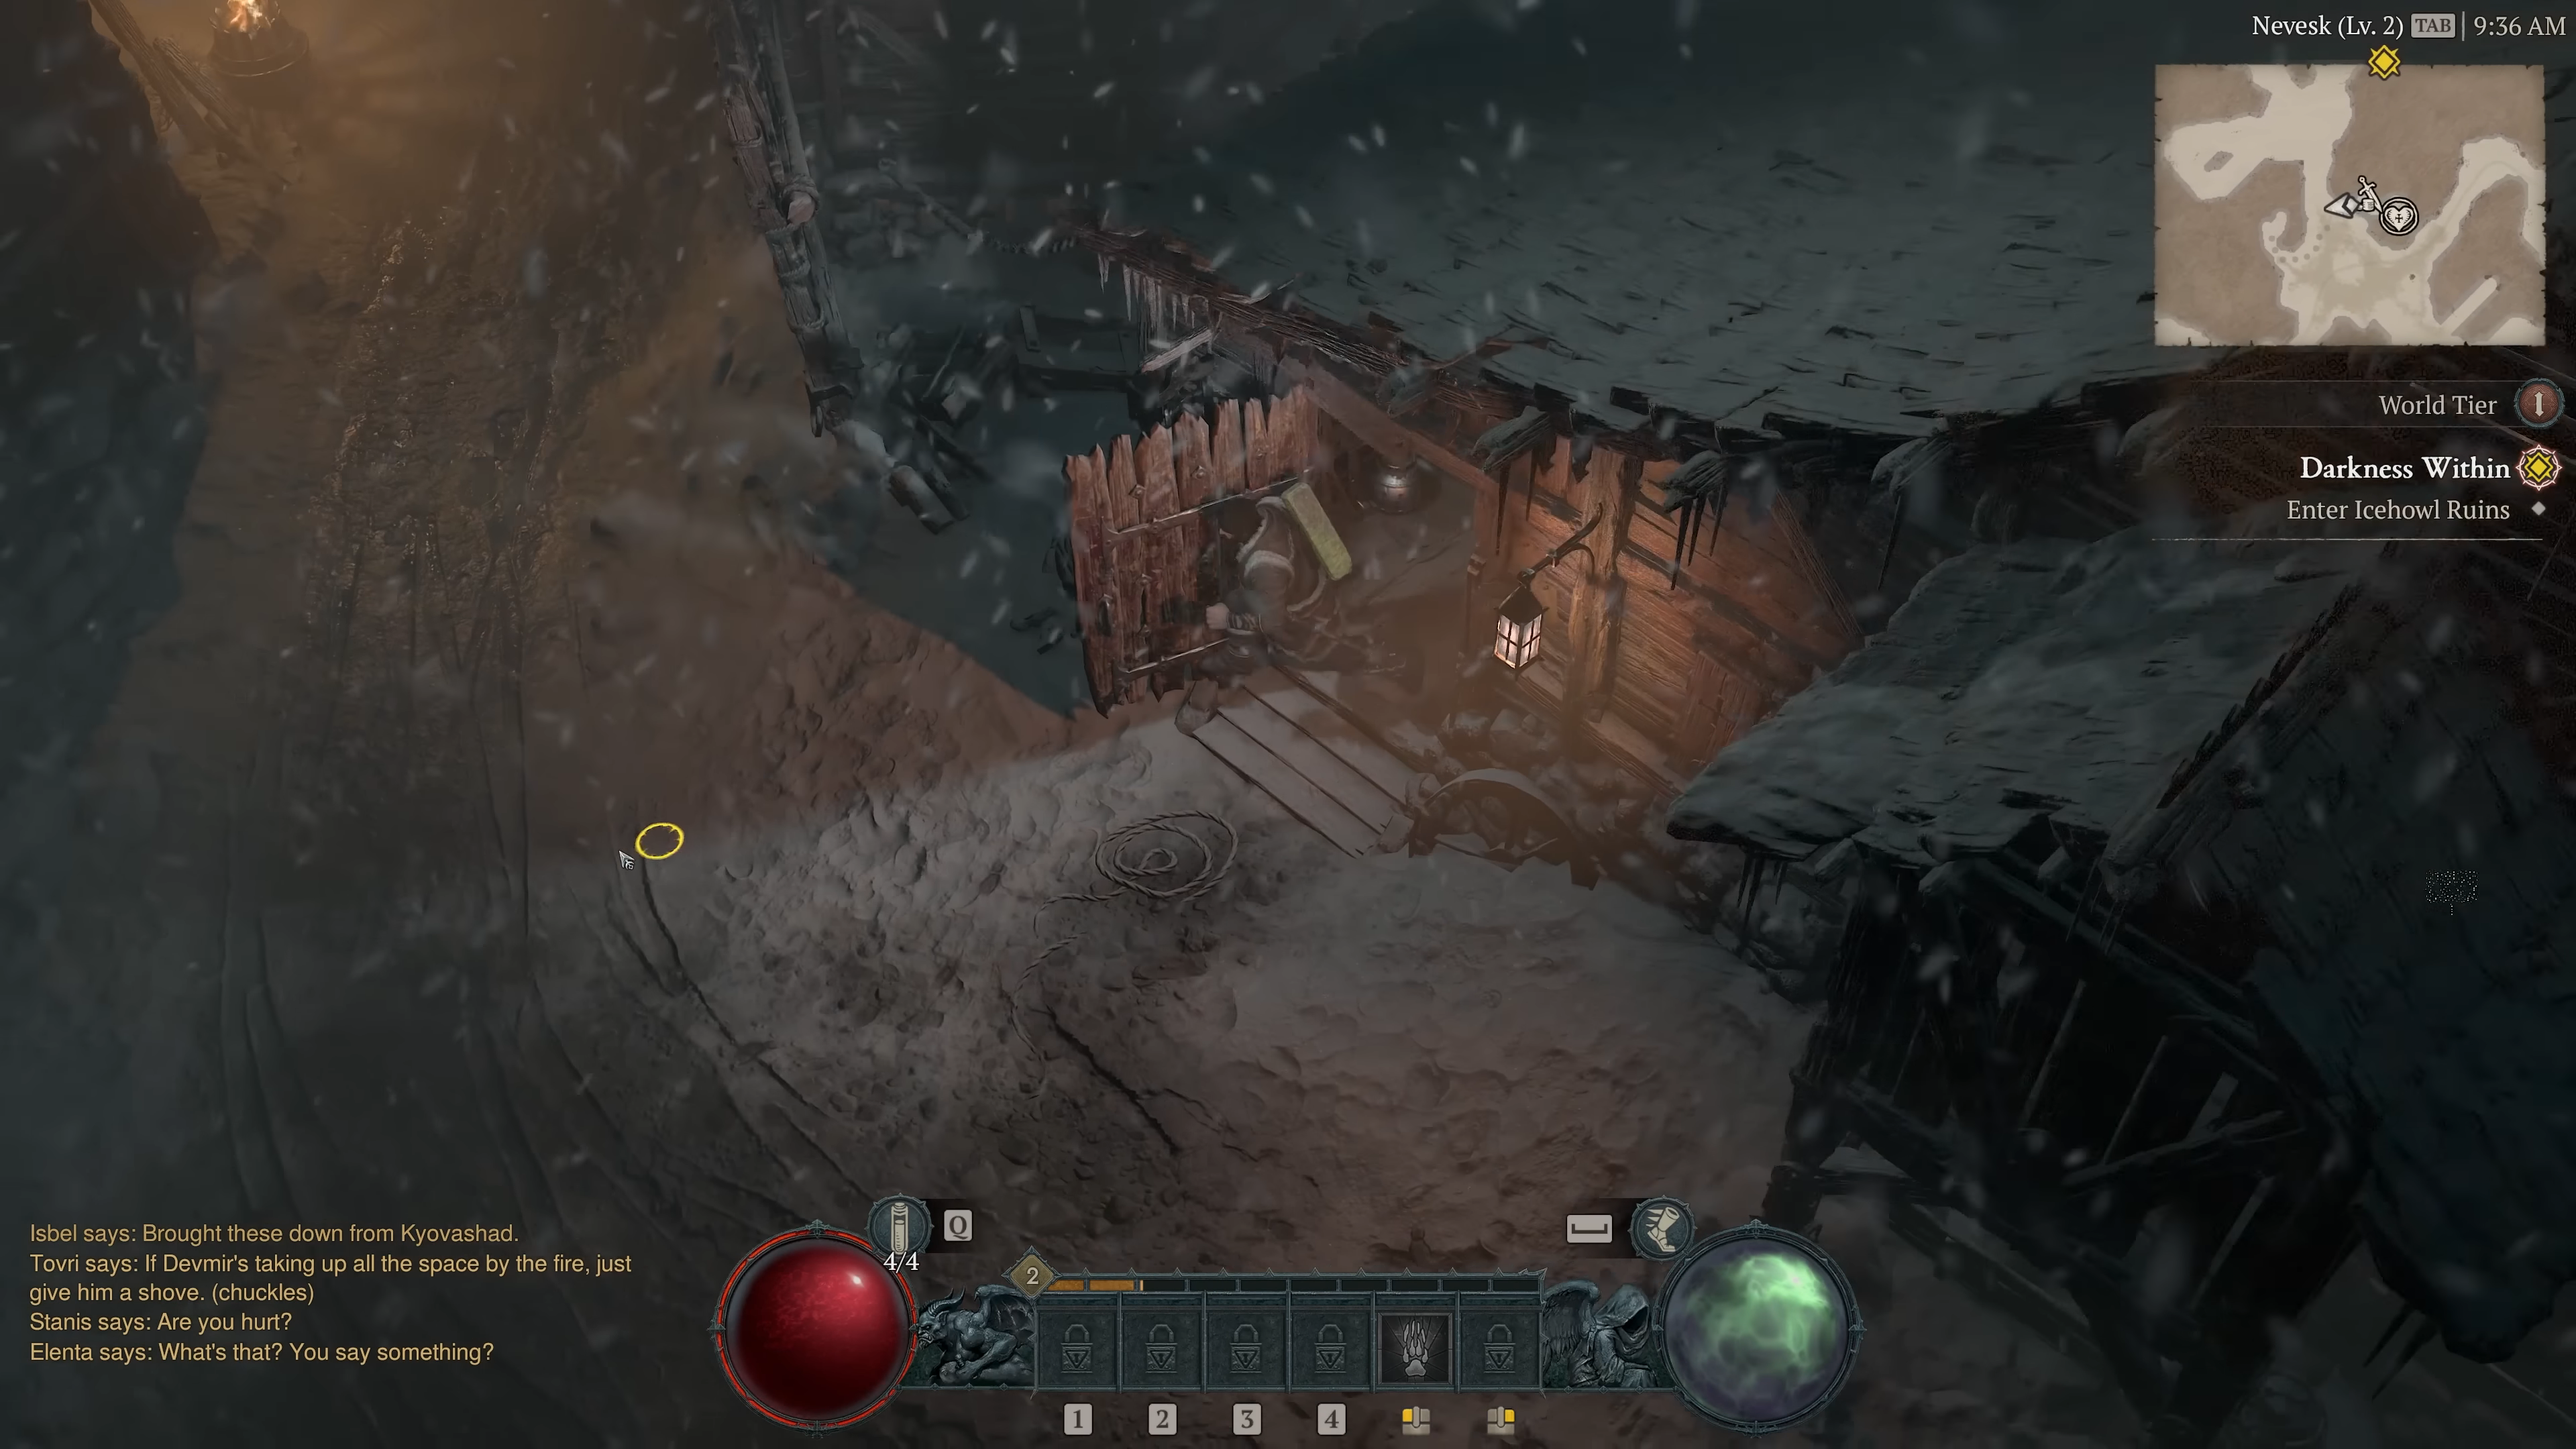
\includegraphics[width=\textwidth]{diablo_outside}
			\caption{Visão externa da casa.}\label{fig:fade_out_example:b}
		\end{subfigure}
		\caption{Transparência de obstáculos em Diablo IV (2023). Fonte: \cite{diablo-game}}\label{fig:fade_out_example}
	\end{figure}

	\item[Sombras de Queda] Os jogos isométricos utilizam da verticalidade para criar profundidade e
	complexidade espacial. Em jogos como Super Mario RPG (1996), a sombra do personagem não segue
	rigorosamente o ângulo da luz do sol do cenário. Em vez disso, há uma sombra projetada diretamente
	no plano do chão abaixo dele. Conforme o personagem pula, a sombra permanece estática no solo, e a
	distância entre o personagem e sua sombra indica visualmente a sua altura atual.

	\begin{figure}[H]
		\centering
		\begin{subfigure}{0.48\textwidth}
			\centering
			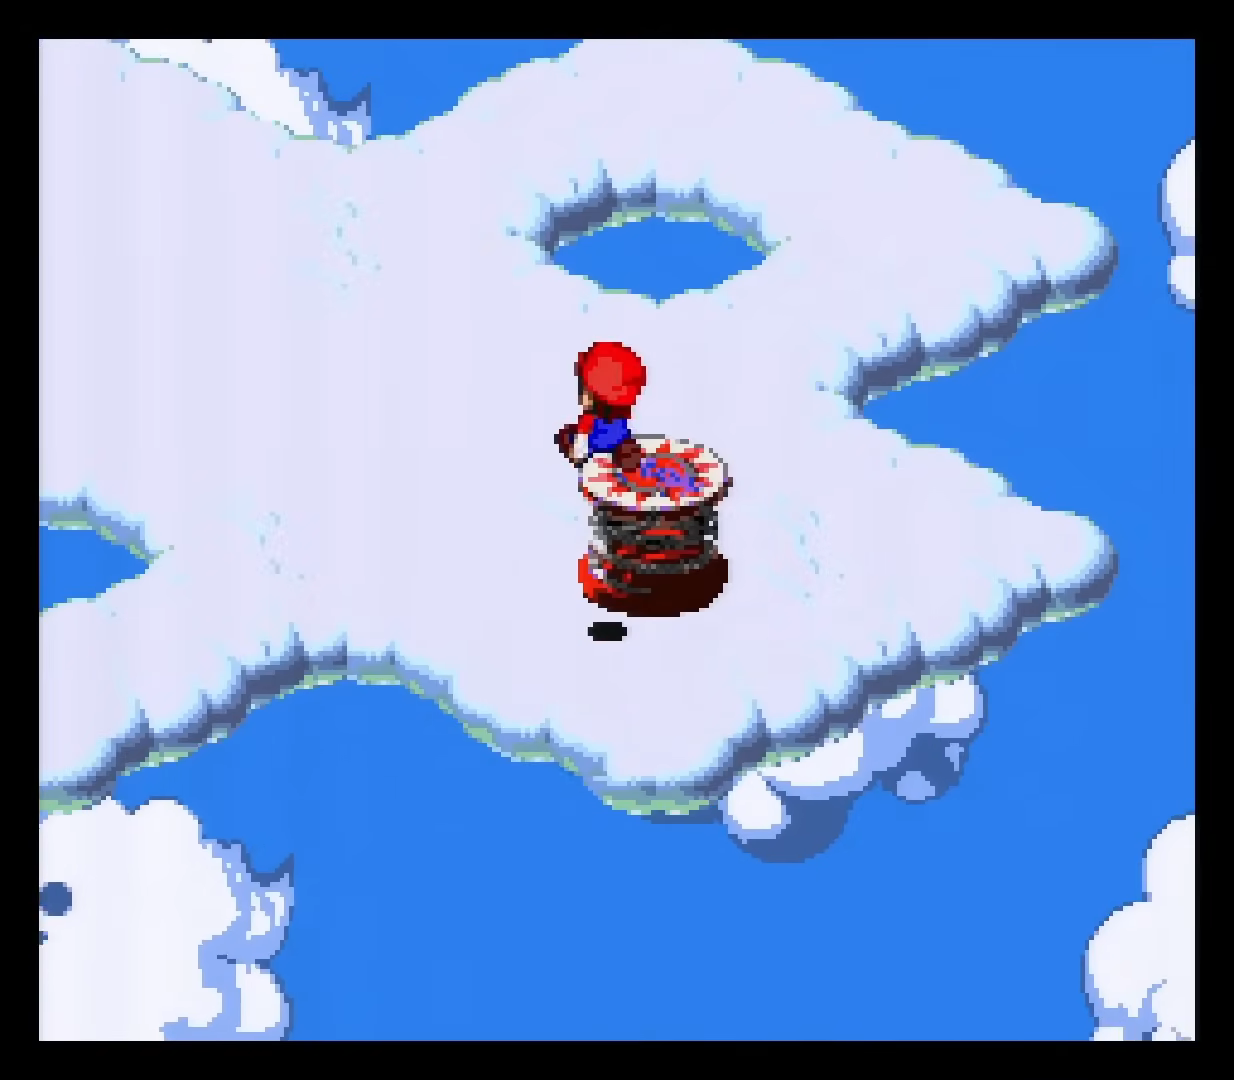
\includegraphics[width=\textwidth]{mario_distant}
			\caption{Personagem em posição elevada.}\label{fig:drop_shadow_example:a}
		\end{subfigure}
		\begin{subfigure}{0.48\textwidth}
			\centering
			
\includegraphics[width=\textwidth]{mario}
			\caption{Personagem em posição baixa.}\label{fig:drop_shadow_example:b}
		\end{subfigure}
		\caption{Sombra de queda em Super Mario RPG (1996). Fonte: \cite{mario-game}}\label{fig:drop_shadow_example}
	\end{figure}
\end{description}

\section{\textit{Low Poly}}
\label{sec:low_poly}

A identidade visual de um jogo 3D é fortemente influenciada pelo nível de detalhamento
geométrico de seus modelos. O termo \textit{low-poly} refere-se à prática de representar objetos
tridimensionais utilizando um número reduzido de polígonos (primariamente triângulos e
quadriláteros) em suas malhas poligonais (\textit{meshes}).

Do ponto de vista da computação gráfica, a redução da contagem de vértices e polígonos
diminui drasticamente o custo de processamento na etapa de transformação geométrica e
rasterização da GPU. Historicamente adotada como solução obrigatória para garantir taxas de
quadros aceitáveis em hardwares restritos, a modelagem \textit{low-poly} se tornou, eventualmente,
uma escolha artística comumente presente em jogos de desenvolvedores independentes devido a
sua simplicidade e eficiência.

Para efeitos comparativos, nos anos 1990 o Playstation 1 prometia a renderização de até 360.000
polígonos por segundo em testes de laboratório, mas na prática os jogos renderizavam entre 90.000 a
180.000 polígonos por segundo devido ao custo de processamento de texturas, shaders, etc. Nesta época,
um personagem costumava ter entre 400 a 800 polígonos dependendo de como o ambiente do jogo era
renderizado. A Lara Croft, protagonista do jogo \textit{Tomb Raider} (1996), possuía cerca de 250 polígonos em
seu modelo original.

\begin{figure}[H]
	\centering
	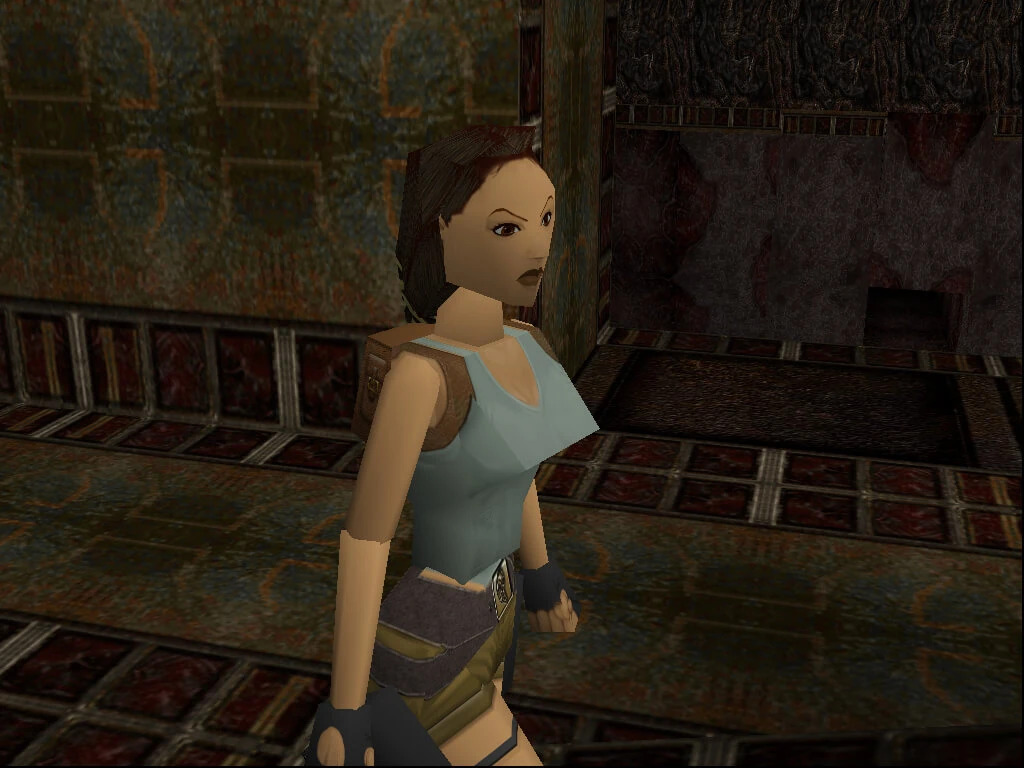
\includegraphics[width=0.6\textwidth]{tomb-raider-1996}
	\caption{Lara Croft (1996). Fonte: \cite{lara-croft-low}}\label{fig:lara_croft_low}
\end{figure}

Em \textit{Tomb Raider: Underworld} (2008), já no Playstation 3, a quantidade de polígonos em
seu modelo aumentou para 32,816, entrando para o \textit{Guinness World Records} como a personagem de video-game mais
detalhada da época.

\begin{figure}[H]
	\centering
	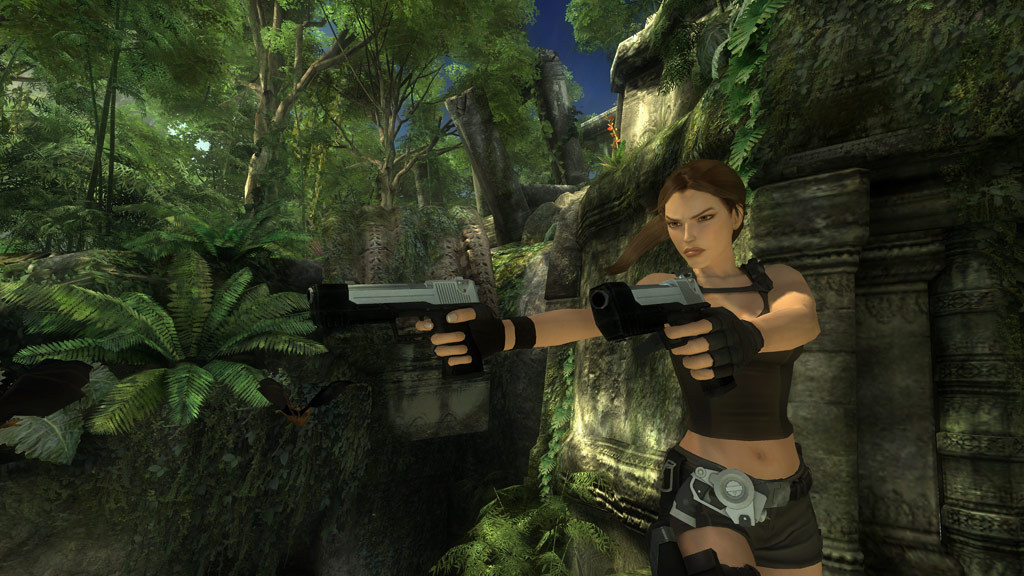
\includegraphics[width=0.6\textwidth]{tomb-raider-2008}
	\caption{Lara Croft (2008). Fonte: \cite{lara-croft-high}}\label{fig:lara_croft_high}
\end{figure}

Em 2017, Johan Lithvall compartilhou sobre sua participação no desenvolvimento do jogo
\textit{Horizon Zero Dawn} (2017) para Playstation 4, onde ficou encarregado do cabelo da protagonista
Aloy, e divulgou que ele possui cerca de 100.000 polígonos, mais que o triplo da quantidade de
um personagem inteiro de 2008.

\begin{figure}[H]
	\centering
	
\includegraphics[width=0.3\textwidth]{aloy}
	\caption{Cabelo da Aloy (2017). Fonte: \cite{aloy}}\label{fig:aloy}
\end{figure}

Os modelos \textit{low poly} facilitam etapas do \textit{pipeline} de produção como Mapeamento UV
para as texturas, o \textit{rigging} (estruturação do esqueleto dos modelos), e animação.
pois com uma menor quantidade de polígonos, menor a necessidade de ponderações de peso, deformações
e poses extremamente complexas, simplificando os movimentos dos personagens.

No contexto artístico, o \textit{low-poly} se destaca por sua abstração geométrica, pois ao
dispensar texturas de alta resolução e malhas densas (\textit{high-poly}), os artistas utilizam
a própria estrutura dos polígonos para definir volumes, silhuetas e superfícies. Essa
abordagem é frequentemente combinada com técnicas de sombreamento plano (\textit{flat shading}),
onde as normais de iluminação são calculadas por face e não por vértice, acentuando as
arestas e proporcionando um aspecto visual limpo e estilizado.

Além disso, a união de modelos \textit{low-poly} com texturas pixelizadas (que é a proposta adotada neste
projeto) gera uma atmosfera estética que se assemelha aos jogos eletrônicos clássicos, reinterpretando-a
com ferramentas tridimensionais modernas. Essa linguagem visual não apenas reforça a legibilidade
espacial exigida por dinâmicas de jogo aceleradas, mas também reduz o consumo de memória de vídeo (VRAM),
permitindo que a capacidade de processamento seja direcionada para a estabilidade da física e para a
fluidez das interações no cenário.

\section{\textit{Fast-Paced}}
\label{sec:fast_paced}

Diferente de jogos focados em exploração de paisagens ou turnos estratégicos,
os jogos \textit{fast-paced} priorizam a velocidade e exigem do jogador respostas
motoras rápidas, reflexos apurados e tomadas de decisão instantâneas em meio a
sequências de ações.

Sob a ótica do \textit{game design}, o desenvolvimento de um jogo \textit{fast-paced} impõe
desafios à engenharia de movimentação e à arquitetura de colisão. Elementos como aceleração,
desaceleração, inércia e transições de animação precisam ser ajustados para eliminar qualquer
sensação de atraso (\textit{input lag} ou lentidão de resposta). O personagem deve responder
de forma imediata aos comandos do usuário, permitindo manobras fluidas como deslizes por
superfícies, saltos e desvios de projéteis.

Além disso, o ritmo do jogo está diretamente atrelado à clareza do \textit{level design}. Em cenários
dinâmicos, o jogador não pode perder tempo tentando entender o espaço ao seu redor. A arquitetura dos
mapas e os elementos visuais devem comunicar instantaneamente as rotas de fuga, os perigos e a posição
dos inimigos.

Assim, a combinação da estética \textit{low-poly} pixelizada e a projeção isométrica atuam de forma
sinergética com o gênero, pois ao remover ruídos visuais complexos e texturas fotorrealistas pesadas,
a cena torna-se limpa, garantindo a legibilidade espacial necessária para que o jogador possa agir e
reagir de forma fluida e sem comprometer o desempenho computacional.

